\documentclass[12pt,a4paper]{extarticle}

\usepackage[latin1]{inputenc}
\usepackage[T1]{fontenc}
\usepackage{lmodern}
\usepackage[french]{babel}
\usepackage{graphicx}
\usepackage{xcolor}
\usepackage{listings}

\definecolor{mGreen}{rgb}{0,0.6,0}
\definecolor{mGray}{rgb}{0.5,0.5,0.5}
\definecolor{mPurple}{rgb}{0.58,0,0.82}
\definecolor{backgroundColour}{rgb}{0.95,0.95,0.92}

\lstdefinestyle{CStyle}{
    backgroundcolor=\color{backgroundColour},   
    commentstyle=\color{mGreen},
    keywordstyle=\color{blue},
    numberstyle=\tiny\color{mGray},
    stringstyle=\color{mPurple},
    basicstyle=\footnotesize,
    breakatwhitespace=false,         
    breaklines=true,                 
    captionpos=b,                    
    keepspaces=true,                 
    numbers=left,                    
    numbersep=5pt,                  
    showspaces=false,                
    showstringspaces=false,
    showtabs=false,                  
    tabsize=2,
    language=C
}


\usepackage[bookmarks]{hyperref}

\FrenchFootnotes{}
\title{\Huge{\textbf{ENSEIRB-MATMECA}\\\Huge{\textbf{1A Informatique 2020-2021}}} \newline \newline \newline \newline \newline \newline \textbf{\Huge{RAPPORT DE PROJET  :} \newline \centering Les tuiles de Wang}}
\author{\textsc{NASDAMI Quatadah} \\ \textsc{ROGER Ga\"etan} \\Encadrant : \textbf{Maxime Poret}}
\date{\today}
\makeatletter

\begin{document}
\begin{figure}[t]
    \centering
    
\includegraphics[height=3cm]{img/logo}
\end{figure}
    \maketitle
    \newpage
    \tableofcontents
    \newpage
    
 
    \section{{Introduction du sujet}}
    \subsection{Pr\'esentation du sujet}
    Le sujet du projet consiste \`a cr\'eer un jeu se basant sur les pavages de Wang. Ce pavage est constitu\'e de tuiles carr\'ees
    ayant chacun de leurs c\^ot\'es associ\'ee une couleur.
    \begin{figure}[h!]
        \centering
        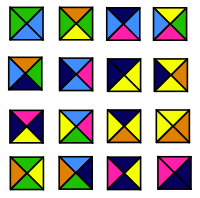
\includegraphics{img/tuile}
        \caption{https://images.math.cnrs.fr}
    \end{figure}
    
    De plus le placement de ces tuiles doit ob\'eir a la contrainte suivante : \\ \textit{Si deux tuiles sont adjacentes leurs cot\'es en commun doivent \^etre associ\'es \`a la m\^eme couleur}.
    \begin{figure}[h!]
        \centering
        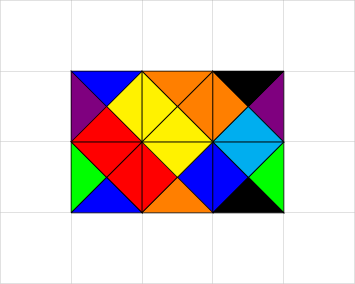
\includegraphics[height=5cm]{img/tuile2}
        \caption{https://www.fil.univ-lille1.fr}
        \label{Wang}
    \end{figure}

    \subsubsection{Achiev0: Version de base}
    Dans cette version, chaque joueur poss\`ede des tuiles distribu\'ees de mani\`ere al\'eatoire. Le but de chaque joueur serait de se d\'ebarasser de toutes les tuiles qu'il poss\`ede pour gagner en les posant 
    sur le plateau en respectant les r\`egles cit\'ees auparavant.
    
    \subsubsection{Achiev1}
    Dans cette version, les joueurs cherchent \`a cr\'eer des motifs rapportant chacun un nombre de points, le gagnant est celui ayant le maximum de points.
    \\ \\ \textbf{exemple :}
    \begin{figure}[h!]
        \centering
        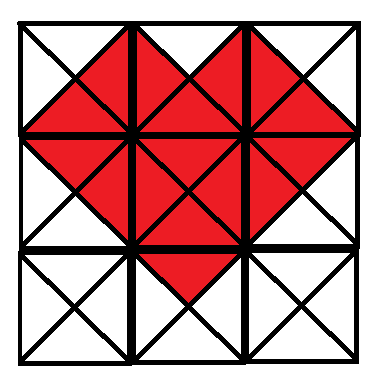
\includegraphics[height=5cm]{img/heart}
        \caption{Motif : heart}
    \end{figure}

    \subsection{Probl\'ematique}
    \begin{itemize}

    \item Impl\'ementation des diff\'erents objets manipul\'es durant la boucle de jeu, \`a savoir les joueurs, les tuiles, le plateau .. etc. 
    \item Analyse des diff\'erentes \'etapes successives n\'ecessaires \`a la boucle de jeu. 
    
    \end{itemize}
    \newpage
    \section{Impl\'ementation du sujet}
    \subsection{Pr\'esentation des algorithmes}
    \subsubsection{Pr\'esentation g\'en\'erale de la boucle de jeu}
    Nous pouvons repr\'esenter le programme par diff\'erentes \'etapes \`a l'aide du sch\'ema suivant :
    \begin{figure}[h!]
        \centering
        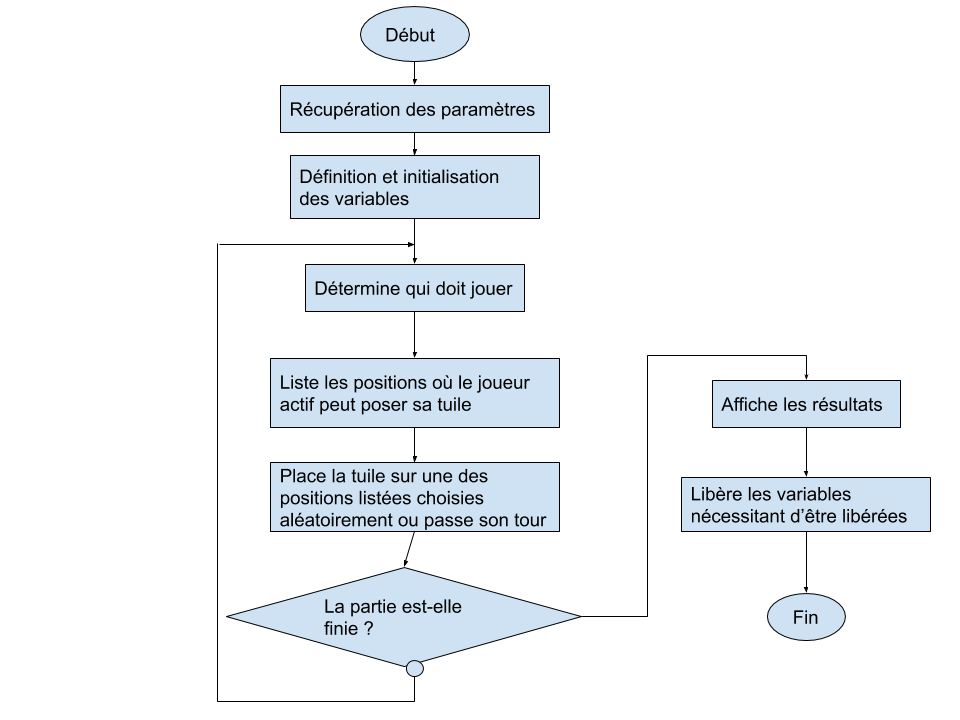
\includegraphics[height=10cm]{img/schemafonctionnel}
        \caption{sh\'ema fonctionnel de la boucle de jeu}
    \end{figure}
    
    Tout d'abord le programme commence par lire et stocker les param\`etres (le nombre de joueurs, la taille du plateau et la seed permettant de g\'en\'erer l'al\'eatoire). 
    Si ces param\`etres ne sont pas renseign\'es, le programme leur attribut des valeurs par d\'efaut.
    
    Ensuite les variables appel\'ees au cours du jeu sont d\'efinies et initialis\'ees. \`A partir de ce moment le jeu est initialis\'e, les tuiles ont \'et\'e 
    distribu\'e entre les joueurs et la partie peut donc commencer.
    
    Pour ce premier tour de jeu, le premier joueur place la premi\`ere tuile de sa main sur une case al\'eatoire du plateau. On teste ensuite si la partie est termin\'ee,
    si elle ne l'est pas on passe au joueur suivant. Pour ce tour on liste toutes les positions o\`u le joueur peut jouer la premi\`ere tuile de sa main puis il la place
    sur l'une de ces positions al\'eatoirement. Si il ne pouvait pas jouer cette tuile, il passe son tour. On teste ensuite si la partie est termin\'ee, si elle ne l'est pas 
    on recommence ces op\'erations en passant au prochain joueur.
    
    La partie se termine lorsque un joueur a fini de poser toutes ses tuiles ou si tous les joueurs on pass\'e leur dernier tour.
    
    Une fois la partie termin\'ee, le programme calcule et affiche les scores des joueurs puis affiche ensuite le gagnant de la partie. Finalement, il lib\`ere l'espace 
    m\'emoire allou\'e durant l'initialisation des variables.


    \subsubsection{Impl\'ementation des structures}
    Etudions maintenant les diff\'erents objets que nous manipulons dans ce projet ainsi 
    que la mani\`ere dont ils sont impl\'ement\'es.
    \newline \\
    Une \emph{couleur} est d\'efinie comme deux cha\^ines de caract\`eres, une repr\'esentant 
    son nom et l'autre son code.


    \begin{lstlisting}[style=CStyle]
struct color{
    const char name[MAX_STR];
    const char code[MAX_STR];
  }; \end{lstlisting}
    
    
    
    Une \emph{tuile} est d\'efinie comme un tableau de 4 pointeurs de couleurs, 
    un pour chaque directions (Nord,Sud,Est,Ouest). 
    Nous utilisons des pointeurs et non directement les couleurs elles m\^emes pour 
    pouvoir changer l'impl\'emenation des couleurs sans impacter l'impl\'emenation des tuiles.
     Pour cette m\^eme raison tous les autres objets utiliseront des pointeurs de tuiles et 
     de couleurs et non les objets eux m\^eme.
    

     \begin{lstlisting}[style=CStyle]
struct tile {
    struct color* tile_colors[4];
  }; \end{lstlisting}
     
     
    Nous devions ensuite cr\'eer une structure file. Pour cela nous avons impl\'ementer 
    une liste simplement cha\^in\'ee FIFO (First In First Out). Cette liste est impl\'ement\'ee de la mani\`ere suivante :
    On d\'efinit d'abord une structure \emph{Element} qui contient l'adresse d'une tuile et l'adresse d'un autre \emph{Element}(suivant). Ainsi on peut passer d'un Element 
    \`a un autre et donc d\'efinir une cha\^ine d'Element.
    On d\'efinit alors la structure \emph{Queue} qui contient l'adresse du premier Element de la file (le prochain Element qui sera supprim\'e de la file) et \`a
     l'aide du cha\^inage pr\'ec\'edemment d\'ecrit on peut donc remonter \`a tout les \'el\'ements de la file. Le dernier \emph{Element} de la file (le dernier \'element 
     ajout\'e \`a la file) renvoie vers l'adresse NULL. Ainsi on sait qu'on se trouve \`a la fin de la file.
    Ces files repr\'esenteront les mains des joueurs.\newpage
    
    \begin{figure}[h!]
        \centering
        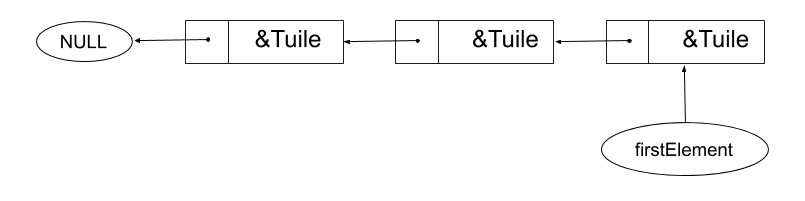
\includegraphics[height = 5cm,width= 12cm]{img/schemafile}
        \caption{sh\'ema d'une file FIFO simplement chain\'ee}
    \end{figure}
    Nous avons ensuite cr\'ee une structure \emph{board} repr\'esentant le plateau de jeu. Cette structure est compos\'e d'une matrice d'adresse de tuiles repr\'esentant 
    les tuiles sur le plateau. On consid\`ere que cette adresse est NULL si aucune tuile n'est pos\'ee \`a cette position. La structure est aussi compos\'ee d'un 
    entier \textbf{size} qui indique la taille d'un c\^ot\'e du plateau (le plateau \'etant un carr\'e).  


    \begin{lstlisting}[style=CStyle]
struct board{
  const struct tile* places[MAX_BOARD_SIZE][MAX_BOARD_SIZE];
  int size;
}; \end{lstlisting}
    
    
    La structure \emph{positions} permet de repr\'esenter une liste de positions du plateau. Elle se compose d'une liste d'abscices, une liste d'ordonn\'ees ainsi qu'un 
    \textbf{entier} indiquant le nombre de positions list\'ees.
    

    \begin{lstlisting}[style=CStyle]
struct positions{
  int i[MAX_BOARD_SIZE*MAX_BOARD_SIZE];
  int j[MAX_BOARD_SIZE*MAX_BOARD_SIZE];
  int length;
}; \end{lstlisting}
    
    
    La structure \emph{player} repr\'esente un joueur. Elle se compose de l'adresse d'une file repr\'esentant sa main, d'un entier repr\'esentant son score ainsi qu'une 
    structure positions d\'efinissant les positions du plateau o\`u le joueur \`a poser une de ses tuiles.
    

    \begin{lstlisting}[style=CStyle]
struct player{
  Queue *cards;
  int score;
  struct positions playertiles;
}; \end{lstlisting}
    
    
    La structure \emph{players} repr\'esente l'ensemble des joueurs. Elle se compose d'une liste de player repr\'esentant les joueurs, un entier indiquant le nombre de 
    joueurs ainsi qu'un entier indiquant le le joueur actif de ce tour.
    

    \begin{lstlisting}[style=CStyle]
struct players{
  struct player player[MAX_PLAYERS];
  int length;
  int rank;
}; \end{lstlisting}
    
    
    La structure \emph{motif} repr\'esente les formes que doivent cr\'eer les joueurs \`a l'aide d'une m\^eme couleur pour obtenir des points. Ces motif sont impl\'ement
     par une taille, le score qui lui est associ\'e  ainsi qu'une matrice de tuile d\'efinissant le motif. Cette matrice contient des tuiles compos\'ees 
     des couleurs \emph{noir} et \emph{blanche}. Les zones blanches de ces tuiles repr\'esentent les zones appartenant au motif.
    

     \begin{lstlisting}[style=CStyle]
struct motif{
    struct tile motiff[MAX_MOTIF][MAX_MOTIF];
    int distance;
    int score_motif;
    int rank;
}; \end{lstlisting}
     
     
    Les objets couleur, tuile, motif et file poss\`edent (avec les fonctions qui leurs sont associ\'ees) chacune leur propre fichier. Toutes les autres structures
    se trouvent dans un m\^eme fichier \emph{player.c}
    \newline \\
    Ainsi on peut constater des d\'ependances entre les diff\'erents fichiers :
    \begin{figure}[h!]
        \centering
        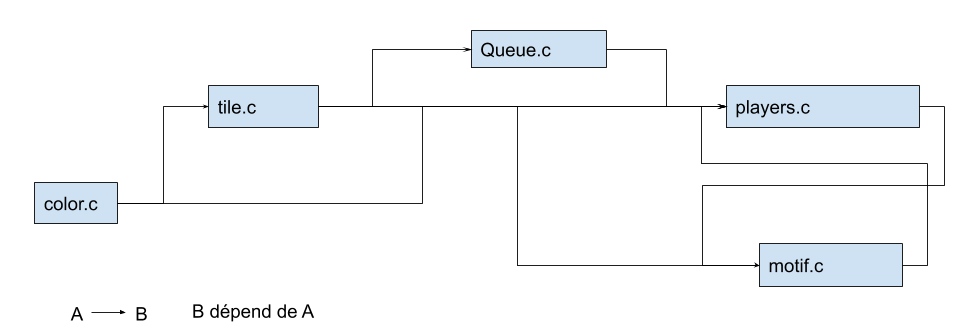
\includegraphics[height=6cm,width=15cm]{img/schemadependance}
        \caption{sh\'ema des d\'ependance entre les fichiers}
    \end{figure}
    \subsubsection{Analyse des fonctions clefs}
    La plupart des fonctions que nous avons d\^u impl\'ementer dans ce projet sont assez simples et f\^urent facilement impl\'ement\'ees. Cependant, d'autres fonctions qu'on qualifierait  
    clefs ont n\'ecessit\'e plus de r\'eflexion et donc une analyse plus appronfondie.
    \newline \\
    La fonction \emph{split\_deck()} prend en argument un deck ainsi que les joueurs et doit distribuer al\'eatoirement les tuiles du deck entre les joueurs. 
    Pour cela nous avons d'abord d\'etermin\'e combien de tuiles chaque joueur devait obtenir. Ensuite pour chaque tuile du deck nous d\'eterminons 
    al\'eatoirement un joueur \`a qui donner celle-ci. Si il \`a d\'ej\`a toutes ses tuiles on la donne au joueur suivant et ainsi de suite.
    \newline \\
    La fonction \emph{list\_authorized\_positions()} prend en argument une tuile \`a poser ainsi que le plateau de jeu et doit retourner la liste des 
    positions o\`u le joueur peut poser cette tuile. Pour cela nous parcourrons chaque case du plateau et nous testons si la tuile peut \^etre poser dans cette case.
    Pour cela nous testons d'abord si la case est vide, puis nous v\'erifions que cette case est adjacente a au moins une tuile d\'ej\`a pos\'ee. 
    Enfin nous testons si mettre la tuile \`a cette case respecte la contrainte du pavage de Wang(~\ref{Wang}). Si cette case remplit toutes 
    ces conditions on l'ajoute \`a la liste des positions authoris\'ees. De plus si toutes les cases sont vides (le premier joueur n'a pas 
    encore jou\'e) toutes les positions du plateau sont ajout\'ees \`a la liste des positions.
    \newline \\
    La fonction \emph{display\_result()} prend en argument le plateau \`a la fin de la partie et la liste des joueurs et renvoie les scores des joueurs. 
    Pour cela nous commen\c ons par parcourir la liste des joueurs. Pour chaque joueur nous parcourons ensuite la liste des tuiles qu'ils ont
     plac\'e sur le plateau. Pour chacune de ces tuiles nous testons si elles appartiennent \`a un motif. Pour tester cela nous commen\c ons 
     pour chaque motif par regarder si la tuile ne se trouve pas trop pr\`es d'un bord du plateau. Ensuite nous testons si la tuile et toutes 
     les tuiles autour de celle ci forment bien le motif. Pour cela on regarde si toutes les zones devant appartennir au motif sont bien de la 
     m\^eme couleur. Enfin si le motif est d\'etect\'e alors on incr\'emente les points du joueurs et on passe \`a sa tuile suivante.
    
    Apr\`es avoir parcouru toute la liste des joueurs de cette fa\c on nous affichons leurs score ainsi que le(s) gagnant(s).

    \subsection{Difficult\'es  rencontr\'ees}
    Au cours de ce projet nous avons rencontr\'e plusieurs obstacles techniques qui nous ont demand\'es d'effectuer 
    des recherches allant au-del\`a de nos acquis.
    
    Le premier de ces obstacles fut l'impl\'emenation de la fonction deck\_init. Cette fonction nous a pos\'e deux probl\`emes. 
    Le premier est le fait que ayant pour contrainte de ne pas modifier color.h, nous n'avions pas acc\`es \`a la structure 
    de color ce qui rendait la cr\'eation des tuiles du deck impossible. Le deuxi\`eme fut que les tuiles \'etaient d\'efinies
     comme des variables locales de deck\_init et donc \'etaient inutilisables dans le reste du jeu.
    \newline
    Le deuxi\`eme obstacle que nous ayons rencontr\'e fut les erreurs de segmentations. Ce fut vraiment un probl\`eme \`a cause 
    du temps que nous avons due prendre pour pouvoir identifier et corriger ces erreurs.
    \newline
    Enfin la derni\`ere difficult\'e \`a laquelle nous avons \'et\'e confront\'e fut la correction de notre codes. M\^eme si notre code 
    \'etait syntaxiquement correct, nos tests n'\'etaient pas coh\'erents avec nos attentes et identifier les erreurs dans notre 
    code fut une t\^ache difficile.
    \subsection{R\'eactions face \`a ces difficult\'es}
	Pour surmonter ces obstacles nous avons cherch\'e des m\'ethodes et d\'ecouvert des outils utiles.
    
    Pour r\'egler le premier probl\`eme avec la fonction deck\_init nous avons simplement utilis\'e la fonction color\_from\_name
     pour avoir acc\`es aux adresses des couleurs sans avoir \`a en d\'efinir. Mais nous avions mis anormalement longtemps avant 
     de comprendre l'int\'er\^et de cette fonction.
    Pour le second probl\`eme de deck\_init nous avions d'abord pens\'e \`a utiliser l'allocation dynamique pour pouvoir utiliser 
    les tuiles d\'efinies localement dans deck\_init. N\'eanmoins, nous avons \'et\'e contraint de ne pas utiliser d'allocation dynamique 
    dans color.c et tile.c nous avons donc cre\'e un tableau en guise de variable globale poss\'edant l'ensemble des tuiles du jeu. 
    \newline
    Les probl\`emes d'\'erreurs de segmentations nous ont permis de nous familiariser avec les outils \emph{gdb} et \emph{valgrind} qui nous 
    ont \'et\'e tr\`es utiles durant le d\'ebogage.
    \newline
    Enfin le temps que nous avons pass\'e sur la correction du code montre bien l'importance de tester chaque petite avanc\'e 
    dans le code car le manque de testes au d\'ebut de notre projet nous a bien port\'ee pr\'ejudice plus tard.

    \section{Analyse algorithmique}
    \subsection{Validit\'e des algorithmes}
    Dans cette partie, on va aborder la validit\'e des algorithmes impl\'ement\'es dans le projet
    ainsi que les test faits dans chaque fichier.
    \subsubsection{Les fonctions agissant sur les \emph{couleurs}}
    Comme indiqu\'e dans l'\'enonc\'e, on a bien respecter les nominations de chaque fonction dans ce fichier \`a savoir :
    \textbf{color\_name, color\_cstring, color\_from\_name.} 
    \\ Apr\'es l'impl\'ementation des tests:
    \begin{lstlisting}[style=CStyle][width=20cm]
printf(" ****** test pour le fichier color.c ******\n");
printf("Renvoie le nom de la couleur <Green> : %s  \n",color_name(&Green));
printf("Renvoie le code de la couleur <Black> : %s \n",color_cstring(&Black));
printf("Renvoie le nom de la couleur <Red> appelee a partir de color_from_name : %s\n",color_name(color_from_name("Red")));
    \end{lstlisting}
    Chaque ligne d\'ebutant par \emph{printf} correspond au test d'une fonction, les premiers mots correspondent 
    \`a ce que devrait retourner la fonction puis apr\`es les \emph{":"}, vient le r\'esultat du test de la fonction.\\
    Voici donc le r\'esultat de leurs validit\'es:
     \begin{figure}[h!]
         \centering
         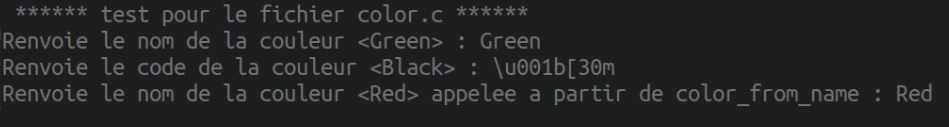
\includegraphics[width=15cm]{img/colorc}
         \caption{rendu du test de \emph{color.c}}
     \end{figure}
     \subsubsection{Les fonctions agissant sur les \emph{tuiles}}
     De la m\^eme mani\`ere que dans color.c, les fonctions de tile.c ont aussi \'et\'e bien pr\'ed\'efinies
     par l'\'enonc\'e.
     Voici l'impl\'ementation de leurs tests:
     \begin{lstlisting}[style=CStyle]
printf("\n\n\n ****** test pour le fichier tile.c ******\n");
struct tile t1 = {{ &Red,&Black,&Black,&Black }};
struct tile t2 = {{ &White,&Red,&White,&White }};
printf("teste empty_tile -> doit renvoyer (0,1) : %d,%d \n",empty_tile()== &t1,empty_tile()==NULL);
printf("teste tile_is_empty -> doit renvoyer (0,1) : %d,%d\n", tile_is_empty(&t1),tile_is_empty(empty_tile()));
printf("teste tile_equals -> doit renvoyer (0,1) : %d, %d \n",tile_equals(&t1,&t2),tile_equals(&t1,&t1)); 
printf("teste tile_edge -> doit renvoyer le nom de la couleur NORD de la tuile t2 : %s\n",color_name(tile_edge(&t2,NORTH)));
     \end{lstlisting}
    Les deux premi\`res lignes correspondent \`a la cr\'eation de deux tuiles pour lesquelles
    on impl\'ement les tests qui suivent.\\
    Les tests sont fait de la m\^eme mani\`ere que dans \emph{color.c}.\\
    Voici le rendu de ces tests : 
    \begin{figure}[h!]
        \centering
        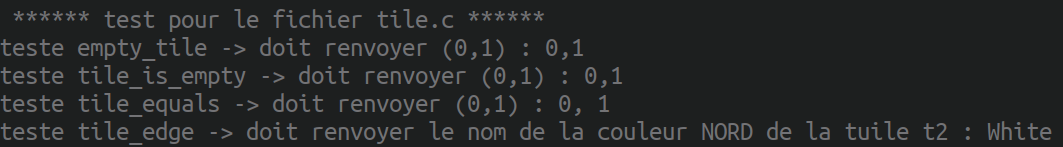
\includegraphics[width=15cm]{img/tilec}
        \caption{rendu du test de \emph{tile.c}}
    \end{figure}
    \\
    De la m\^eme mani\`ere, ce qui vient avant les deux points \emph{':'} correspond \`a ce que doit retourner la fonction
    apr\`es ces deux points.\\
    La fonction \emph{deck\_init} est la moins \'evidente \`a tester 
    comme le montre le code suivant : 
    \begin{lstlisting}[style=CStyle]
struct deck de;
deck_init(&de);
int i = de.size;
int pair = 0;
while(i>0)
{
  printf("[%s",color_name(de.cards[pair].t->tile_colors[0]));
  for (int dir = 1; dir<4;dir ++)
  {
    printf(",%s",color_name(tile_edge(de.cards[pair].t,dir)));
  }
  printf("] : %d fois \n",de.cards[pair].n);
  i -= de.cards[pair].n;
  pair++;
}
printf("La taille du deck est de : %d tuiles \n",de.size);
    \end{lstlisting}
    \paragraph{Les principales \'etapes du test de la fonction \emph{deck\_init} :}
    \begin{itemize}
        \item Appel \`a la fonction \emph{deck\_init}.
        \item Initialisation d'une variable \emph{i} avec la taille du \emph{deck}.
        \item Affichage de toutes les couleurs de chaque tuile tout en d\'ecrementant la variable \emph{i}
        pour la terminaison de la boucle \emph{while}.
        \item Affichage de la taille du \emph{deck}.
    \end{itemize}

    Pour l'initialisation qu'on avait faite, en voici le r\'esultat : 
    \begin{figure}[h!]
        \centering
        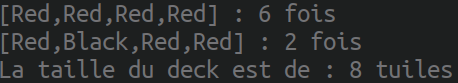
\includegraphics[width = 10cm]{img/deckinitc}
        \caption{rendu du test de \emph{deck\_init}}
    \end{figure}
    \subsubsection{les fonctions agissant sur les \emph{files} ou \emph{mains} des joueurs}
    Il s'agit des tests des fonctions du fichier \emph{queue.c} qui rappelons le, manipulent
    les tuiles dans la main du joueur.
    \begin{itemize}
        \item La fonction \emph{initQueue()} initialise la structure \textbf{Queue} en mettant son premier
         \'el\'ement comme \textbf{NULL}.
        \item La fonction \emph{push()} rajoute un \'el\'ement \`a la file entr\'ee en param\`etres, puis le
        met dans son rang en respectant les r\`egles d'une file.
        \item La fonction \emph{top()} retourne le premier \'l\'ement de la file et la fonction \emph{pop()} 
        se charge de le supprimer.
        \item La fonction \emph{popAll()} supprime tous les \'el\'ements de la file sauf \emph{NULL}
        qui apr\`es suppression devient donc le premier \'el\'ement de la file.
        \item La fonction \emph{rand\_q()} qui sert \`a m\'elanger les tuiles avant de les distribuer.
    \end{itemize}

    L'impl\'ementation des tests donne :
    \begin{lstlisting}[style=CStyle]
printf("\n\n\n ****** test pour le fichier queue.c ******\n");
Queue* q = initQueue();
printf("teste si le premier element de la file est NULL -> doit envoyer 1 : %d\n",q->firstElement == NULL);
push(q,&t1);
push(q,&t2);
printf("teste top -> doit envoyer 1 : %d\n",top(q)->tile == &t1);
pop(q);
printf("teste si t1 a bien ete supprime -> doit envoyer 1 : %d\n\n",top(q)->tile == &t2);
popAll(q); \end{lstlisting}
    Le rendu donne : 
    \begin{figure}[h!]
        \centering
        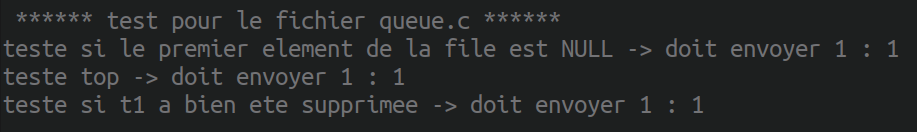
\includegraphics[width=15cm]{img/queue1c}
        \caption{Rendu du test des fonctions de \emph{queue.c}}
    \end{figure}
    \\
En ce qui concerne la fonction \emph{rand\_q()}:

\begin{lstlisting}[style=CStyle]
printf("******test de rand_q******\n");
printf("file non melangee : ");
for (int i =0; i<5; i++)
{
  push(q,&t1);
  printf("t1 ");
}
for (int i =0; i<5; i++)
{
  push(q,&t2);
  printf("t2 ");
}
q = rand_q(q);
printf("\nfile melangee : ");
while (top(q) != NULL)
{
  const struct tile *t = top(q)->tile;
  if (t == &t1)
    printf("t1 ");
  if (t == &t2)
    printf("t2 ");
  pop(q);
}    \end{lstlisting}
    Ce qui donne comme rendu le r\'esultat suivant:
    \begin{figure}[h!]
        \centering
        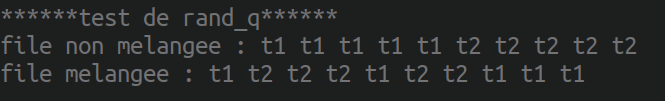
\includegraphics[width=15cm]{img/rand_q}
        \caption{rendu du test de \emph{rand\_q}}
    \end{figure}

    \subsubsection{Le reste des fonctions}
    Le fichier \emph{players.c} comporte toutes les fonctions qui restent et qui sont impl\'ement\'ees dans la boucle
    du jeu. Ces derni\`eres sont directement test\'ees par la boucle du jeu et donc on ne les testera pas dans cette partie.

    \title{\textbf{Remarque:}}
    En ce qui concerne l'\textbf{Achiev1}, on a agit en majeure partie sur la fonction
    \emph{display\_results()}. Le but \'etait de rajouter les scores des motifs aux joueurs les poss\'edant
    et d'afficher le score finale de chaque joueur ainsi que d'afficher le gagnant ou les gagnants de la partie.
    \\Pour tester donc cette nouvelle \emph{display\_results()}, On a limit\'e le boardSize \`a 3x3, et on a laiss\'e un seul joueur,
     puis on lui a distribu\'e 9 tuiles
    semblables remplies de la m\^eme couleur dans toutes les directions. De plus, on sait que pour avoir 
    le motif coeur il faut 7 tuiles de la m\^eme couleur plac\'ees sous forme d'un carr\'e, donc la seule 
    possibilit\'e pour le joueur quelque soit la combinaison avec laquelle il pose ses tuiles, il finira
    par arriver \`a faire le motif coeur et seulement lui. D'o\`u, son score finale sera bien celui du 
    coeur \`a savoir 60.
    \\
    Si on fait pareil pour BoardSize (4 x 4) et on distribuant 16 tuiles \`a l'unique joueur, il finira
    par arriver \`a faire 4 coeurs, son score finale serait donc de 240 = 60 * 4.
    \\
    \begin{lstlisting}[style=CStyle]
// Board size 
unsigned int boardSize = 3;
// number of players in the game
unsigned int playersNumber = 1; \end{lstlisting}
    Le r\'esultat suivant montre bien que la fonction marche : 
    \begin{figure}[h!]
        \centering
        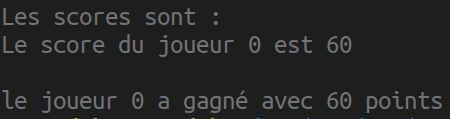
\includegraphics[width=10cm]{img/display}
        \caption{rendu de la fonction \emph{display\_results}}
    \end{figure}



    \subsection{Complexit\'e algorithmique}
    Les fonctions qui viennent dans \emph{color.c} et \emph{tile.c} et \emph{queue.c} sont 
    soit de complexit\'e constante ou lin\'eaire.
    D\`es lors la cr\'eation de la structure \emph{Board} qui contient une matrice de tuiles, les fonctions qui utilisent
    cette structure ont des complexit\'es bien plus elev\'ees puisqu'elles sont dans l'obligation de parcourir le plateau 
    de jeu (qui est une matrice).
    \\
    Dans cette partie on va aborder ces fonctions : 


    \subsubsection{La fonction \emph{list\_authorized\_places()}}
    Cette fonction a pour but, rappelons le, parcourir le plateau de jeu puis retourner une liste de positions dans \emph{struct positions} 
    dans lesquels il est possible pour le joueur actif de d\'eposer une de ses tuiles.
    Cette fonction donc doit :
    \begin{itemize}
        \item Parcourir le plateau qui est pour nous une matrice carr\'ee.
        \item Chercher o\`u est-ce que le joueur pourrait d\'eposer sa tuile entr\'ee en param\`etres, et donc cette \'etape 
        requiert le parcours des 4 directions de sa tuile.
    \end{itemize}
    Ce qui donne en code :
    \begin{lstlisting}[style=CStyle]
...
for (int k=0; k<b->size; k++){
    for (int l=0; l<b->size; l++){
    ...
        for (int dir = 0; dir<4; dir++){
        ... \end{lstlisting}
    La complexit\'e donc de cette fonction est de l'ordre \( C = O((b\rightarrow size)^2 \times 4)\)
    \\ Il s'agit donc d'une complexit\'e \textbf{quadratique}, chose qui \'etait pr\'evue puisque notre \emph{struct board} 
    est sous forme d'une matrice carr\'ee.


    \subsubsection{La fonction \emph{display\_results()} de l'achiev1 :}
    Il s'agit de la fonction ayant la plus grande complexit\'e dans notre jeu et dont nous sommes pas fi\'eres de l'avoir 
    impl\'ement\'e de cette mani\`ere.
    En effet, la fonction a besoin de : 
    \begin{itemize}
        \item Parcourir tous les joueurs
        \item Parcourir les tuiles qu'ils poss\`edent (que les joueurs ont pr\'ec\'edemment d\'epos\'e sur le plateau)
        \item Parcourir la liste des motifs permettant d'obtenir des scores ( 2 dans notre cas, on peut la consid\'erer constante)
        \item Parcourir les cases entourant la tuile centrale du joueur pour v\'erifier si le joueur a r\'eussi \`a faire un motif.
    \end{itemize}

    Ce qui donne finalement : 
    \begin{lstlisting}[style=CStyle]
for (int k=0 ;k < p->length; k++)
    {
      for (int l=0; l < p->player[k].playertiles.length ; l++  )
      {
        for (int m=0 ; m<2 ; m++)
        ...
            for (int a=x-liste_motif[m].distance; a<x+liste_motif[m].distance +1 ;a++)
              {
                for (int z=y-liste_motif[m].distance; z<y+liste_motif[m].distance +1 ;z++)
                {
                  for (int d=0; d<4; d++)
                  ...
                    if (tile_edge(&liste_motif[m].motiff[a-x+liste_motif[m].distance][z-y+liste_motif[m].distance],d) == color_from_name("White")) \end{lstlisting}
    La derni\`ere boucle est de complexit\'e constante, la complexit\'e de cette fonction est de l'ordre de \( O(p \rightarrow length \times playertiles.length \times 2 \times 3 \times 3 \times 4 \times len)  \)
    \\En effet: \\
    Dans l'\'enonc\'e, il est mentionn\'ee que la distance de Chebychev ne doit pas d\'epasser 2, les deux avants derni\`eres boucles utilisent chacune le double de la distance
    de Chebychev(qui est pour notre cas \'egale \`a 1 ) +1, d'o\`u le 3 dans le calcul de la complexit\'e. Le len \`a la fin correspond \`a la complexit\'e de la fonction \emph{color\_from\_name()} qui est 
    lin\'eaire, puisqu'elle utilise la fonction \emph{strcmp} dans une boucle finie.  \
    La complexit\'e finale est donc \textbf{cubique}.

    \section{Bilan}
    \subsection{Rendu finale du jeu}
    Dans cette partie, nous allons pr\'esenter le rendu de la boucle finale du jeu.
    Les \'etapes se d\'eroulent de cette mani\'ere : 
    \begin{enumerate}
        \item Les joueurs re\c oivent chacun des cartes.
        \item La partie commence et le programme entre dans la boucle du jeu
        \item suivant les consignes et r\`egles du jeu, la partie se termine
        \item On affiche les r\'esultats finaux(le score de chaque joueur ainsi que le(s) gagnant(s) de la partie)
    \end{enumerate}
    Lors de l'impl\'ementation de nos fonctions, nous avons pris en compte le fait de mettre \emph{printf} partout l\`a o\`u on a jug\'e qu'il faut le mettre
    pour rendre un peu vivant le rendu du jeu.
    Voici le r\'esultat final pour une boucle de 2 joueurs, un deck de plusieurs tuiles( >100 ) qu'on va pas tout montrer:

    \begin{figure}[h!]
        \centering
        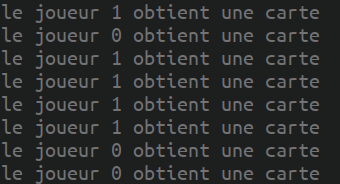
\includegraphics[height=5cm,width=8cm]{img/rendu1}
    \end{figure}

    \begin{figure}[h!]
        \centering
        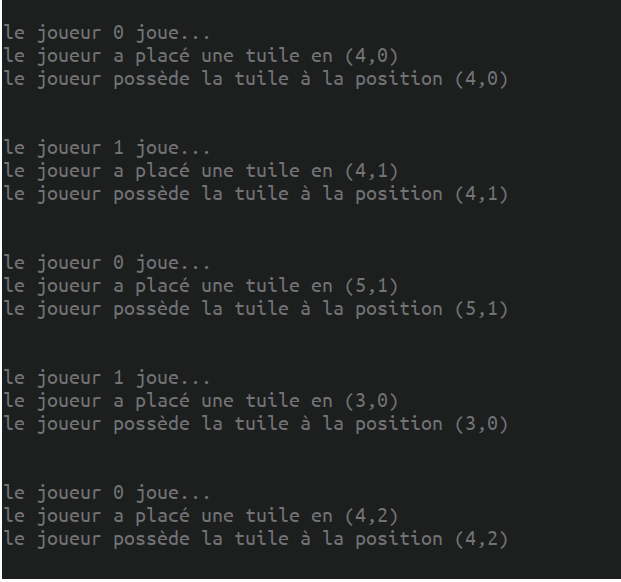
\includegraphics[height=10cm,width=10cm]{img/rendu2}
    \end{figure}

    \begin{figure}[h!]
        \centering
        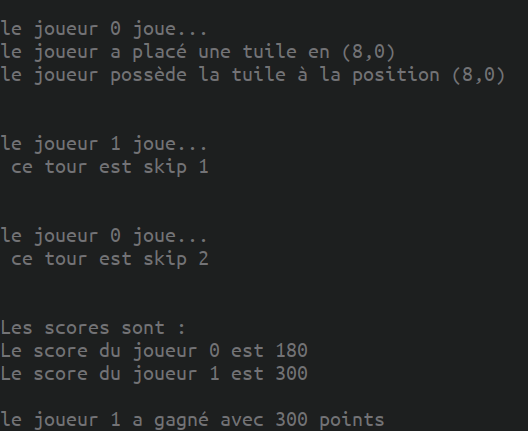
\includegraphics[height=8cm,width=10cm]{img/rendu3}
    \end{figure}

    \subsection{Options de compilation}
    Par d\'efaut, le jeu est mis \`a 2 joueurs, pour un plateau de taille 10 et pour une seed \'egale \`a 0.
    Sauf qu'il existe des options de compilation du jeu avec lesquelles on peut changer ces donn\'ees l\`a \'a savoir une compilation avec \emph{-s} pour changer la valeur
    de la seed, \emph{-n} pour changer le nombre des joueurs et \emph{-b} pour changer la taille du plateau
    \subsection{Conclusion}
    Ce projet de programmation que nous venons de r\'ealiser nous a permis de manipuler tous les acquis du cours et m\^eme aller plus loin que cela en d\'ecouvrant de nouvelles 
    manipulations dans ce monde vaste de \emph{l'informatique} \`a titre d'exemple l'utilisation de \emph{gdb,valgrind}. De plus, nous avons fait face \`a de nombreux probl\`emes qu'on 
    a pu finalement r\'esoudre.

\end{document}

% Introduction du sujet
%   -Pr\'esentation du sujet + probl\'ematique
%   -Mise en place des objectifs
%
% Organisation du travail
%   
% Impl\'ementation du projet
%   -Pr\'esentation des algorithmes
%   -Difficultés rencontrées
%   -Mise en place des solutions

% Analyse algorithmique
%   -Validité des algorithmes
%   -Complexité 
%   -défaut/Amélioration
%
% Bilan
%   -Impressions, ressentis
%   -Conclusion
% 